\RequirePackage[2020-02-02]{latexrelease}
\documentclass{ntuthesis}


\usepackage{amsmath, amssymb, amsthm}
\usepackage{bm, bbm}
\usepackage{physics}
\usepackage{natbib}

\usepackage{appendix}
\usepackage{caption}    % for subfigure
\usepackage{subcaption} % for subfigure
\usepackage[compact]{titlesec}    % remove redundant spacing
\usepackage{times}
\usepackage{threeparttablex,longtable}
\usepackage{booktabs}
\usepackage{afterpage}  % load the afterpage package
\usepackage[inline]{enumitem}   % can get rid of new line
\usepackage{verbatim}
\usepackage{color}
\usepackage{url}
\usepackage{graphicx}
\usepackage{setspace}
\usepackage{array}
\usepackage{wallpaper}
\usepackage[hidelinks]{hyperref}
\usepackage[printwatermark]{xwatermark}
\usepackage[capposition=top]{floatrow}
\usepackage{chngcntr}
\newcommand{\BL}{\emph{Bitcoin Law}}
\newcommand{\chivo}{\emph{Chivo Wallet}}
\newcommand{\BC}{\emph{Bitcoin City}}

\DeclareMathOperator*{\argmin}{arg\,min}

\newcommand{\refeq}[1]{Equation~({\ref{#1}})}
\newcolumntype{H}{>{\setbox0=\hbox\bgroup}c<{\egroup}@{}}


\counterwithout{equation}{chapter}
\counterwithout{figure}{chapter}
\counterwithout{table}{chapter}
% Using the tex-text mapping for ligatures etc.
\defaultfontfeatures{Mapping=tex-text}
% Set the default fonts
\setmainfont{Times New Roman}
\setCJKmainfont[AutoFakeBold=true,AutoFakeSlant=true]{標楷體}
%\setCJKmainfont[BoldFont={粗楷體},ItalicFont={斜楷體}]{標楷體}

\theoremstyle{definition}
\newtheorem{definition}{Definition}

\ifdefined\firstpage

  \def\withwatermark{1}
  \ifdefined\withwatermark
    \newsavebox\mybox
    \savebox\mybox{\tikz[opacity=0.5]\node{
\includegraphics{watermark.pdf}};}
    \newwatermark*[allpages,xpos=6.1725cm,ypos=10.5225cm,scale=0.5]{\usebox\mybox}
  \fi

  % digital object identifier
  \ifdefined\withdoi
    \insertdoi
  \fi
\fi

\makeatletter
\AtBeginDocument{
  \hypersetup{
    pdftitle={\@titleen},
    pdfauthor={\@authoren},
    pdfsubject={\@typeen{} \@classen},
    pdfkeywords={\@keywordsen}
  }
}
\makeatother

% Your information goes here
% author: Tz-Huan Huang [http://www.csie.ntu.edu.tw/~tzhuan]

% ----------------------------------------------------------------------------
% "THE CHOCOLATE-WARE LICENSE":
% Tz-Huan Huang wrote this file. As long as you retain this notice you
% can do whatever you want with this stuff. If we meet some day, and you think
% this stuff is worth it, you can buy me a chocolate in return Tz-Huan Huang
% ----------------------------------------------------------------------------

% Syntax: \var{English}{Chinese}
\university{National Taiwan University}{國立臺灣大學}
\college{College of Social Science}{社會科學院}
\institute{Department of Economics}{經濟學系}
\title{Examining the Chinese Debt-Trap Diplomacy}{檢視中國債務陷阱}
\author{Chia-Wei Chen}{陳家威}
\studentid{R10323045}
\advisor{Tai-kuang Ho, Ph.D.}{何泰寬 博士}
\defenseyear{2023}{112}
\defensemonth{July}{7}
\defenseday{12}
\doi{doi:10.6342/NTU2017XXXXX}
\keywords{Debt-Trap Diplomacy, Belt and Road Initiative, Sovereign Debt, Optimal Default}{債務陷阱外交、一帶一路、主權債務、最適違約決定}


\titleformat{\chapter}                      % 設置 Chapter 格式
{\Huge\bfseries}                            % 定義 format
{Chapter~\thechapter:~}              		        % 定義 label
{1em}                                       % 定義 sep
{} 
\begin{document}

\frontmatter

\makecover

\ifdefined\excludefirstpage

  \def\withwatermark{1}
  \ifdefined\withwatermark
    \newsavebox\mybox
    \savebox\mybox{\tikz[opacity=0.5]\node{
\includegraphics{watermark.pdf}};}
    \newwatermark*[allpages,xpos=6.1725cm,ypos=10.5225cm,scale=0.5]{\usebox\mybox}
  \fi

  % digital object identifier
  \ifdefined\withdoi
    \insertdoi
  \fi
\fi

% \makecertification

% \begin{acknowledgementszh}
感謝\ldots
\end{acknowledgementszh}

\begin{acknowledgementsen}
I'm glad to thank\ldots 
\end{acknowledgementsen}

% \begin{abstractzh}
關於中國在「一帶一路」倡議下向接受國家提供的過度貸款是否導致這些國家陷入高度債務並最終陷入「債務陷阱」的爭議仍然存在。本論文旨在通過運用一個主權債務模型的校準,從實證角度對這個議題進行考察。具體而言,本研究聚焦於兩個在中國戰略上具有重要地位的國家 --- 斯里蘭卡和巴基斯坦。

研究結果確認了這兩個國家在接受大量貸款後確實陷入了債務違約的狀態。基於這些結果,本研究提出了兩個債務陷阱的類別,並將斯里蘭卡和巴基斯坦分別歸入不同的類別。這種分類方法為債務陷阱外交的相關文獻提供了客觀的評估和呈現方式。
\bigbreak
\noindent \textbf{關鍵字:}{\, \makeatletter \@keywordszh \makeatother}
\end{abstractzh}

\begin{abstracten}

    Ongoing debates remain surrounding whether the excessive loans provided by China under the Belt and Road Initiative lead to high indebtedness and eventual ``debt traps'' for recipient countries. This thesis empirically examines this topic through the calibration of a sovereign debt model. Specifically, the study focuses on two strategically important countries --- Sri Lanka and Pakistan.
    The research findings validate the notion that these two countries indeed fell into the default set once they received substantial loan amounts, allowing for two categories of debt traps into which Sri Lanka and Pakistan reside. This categorization offers an objective assessment and presentation method within the literature on debt-trap diplomacy.
    \bigbreak
\noindent \textbf{Keywords:}{\, \makeatletter \@keywordsen \makeatother}
\end{abstracten}

\begin{comment}
\category{I2.10}{Computing Methodologies}{Artificial Intelligence --
Vision and Scene Understanding} \category{H5.3}{Information
Systems}{Information Interfaces and Presentation (HCI) -- Web-based
Interaction.}

\terms{Design, Human factors, Performance.}

\keywords{Region of interest, Visual attention model, Web-based
games, Benchmarks.}
\end{comment}


% \tableofcontents
% \listoffigures
% \listoftables

\mainmatter


\chapter{Introduction}
As China's economic influence continues to grow, its lending practices to developing countries have come under scrutiny.
The concept of ``debt-trap diplomacy'' (hereinafter DTD), whereby China extends excessive loans to countries in exchange for political or economic concessions, has become a topic of heated debate \citep{Chellaney_2017}.
While some argue that the debt-trap problem poses a significant threat to the economic and political stability of vulnerable countries, others contend that it is overstated.

From the political science aspect, an analysis from the Belfer Center for Science and International Affairs states that China utilizes DTD as a technique to achieve strategic objectives, such as projecting power across South Asian trading routes, undermining regional opposition to its South China Sea claims, and supporting its naval efforts to break out into the Pacific \citep*{Parker2018}.
Critics of this phenomenon argue that claims of DTD are often exaggerated or based on incomplete information. For example, \citet*{Brautigam-meme-2020} argues that the debt-trap is based on a flawed understanding of Chinese lending practices and the histories of the target countries, and that China is not strategically pursuing the DTD on developing countries.

The opacity in Chinese lending practices has been a longstanding challenge in the analysis of the DTD problem \citep*{Horn-Reinhart-Trebesch-21}.
The lack of transparency in the Chinese lending system, whereby loan terms, conditions and collateral requirements are not always disclosed to the borrowers, makes it difficult for economists and policymakers to fully grasp the magnitude of the issue.
Therefore, it has been challenging to assess the sustainability of debts of borrowing countries and their ability to service their obligations, as well as the potential impact of China's lending practices on the economy of low income developing countries (LIDC), especially those in the Belt and Road Initiatives (BLI).
As a result, recent studies on whether DTD is a myth have primarily been conducted normatively in the field of political science, rather than a positive economics analysis~\citep[See, e.g.,][]{Himmer2023-vn,Chen2020-eo}.

However, with the emergence of new and detailed data on Chinese lending practices, recent studies have begun to shed light on the nature and implications of the China debt.
In this thesis, I aim to shed light on whether a country fell into the debt-trap by applying a new and detailed data provided by \citet*{Horn-Reinhart-Trebesch-21}, hereinafter referred to the ``HRT database'', on the sovereign debt model proposed by \citet*{Na-18}, to provide insights into the sustainability of the debt of borrowing countries.
By calibrating the model for a particular country, a set of tradable-output levels which would cause the country to default could be obtained, given its current debt level. Following the approach of \citet{Hinrichsen_2020-chapter4}, this set is presented graphically with each data point on the space representing a debt-output pair for a specific year. This visual representation allows for an examination of whether the country has been in the default zone but has managed to avoid default due to other enforcement mechanisms, in this case might be the political leverage from China.

It requires a lot of work to calibrate all countries to match the model, therefore it is optimal to narrow down the sample countries to those that provides the most insight on the DID issie. I consider countries
\begin{enumerate*}
    \item that is constantly receiving loans from other international institutes,
    \item that indicates an increasing amount of debt from China that eventually exceeds other creditors, and
    \item in which China launches large infrastructure programs.
\end{enumerate*}
% \citet*{Hurley19-8-debt-trap} examines the dept-to-GDP ratio versus the share of China's debt, and identifies eight
% countries\footnote{
%     These countries are Djibouti, Kyrgyzstan, Laos, the Maldives, Mongolia, Montenegro, Pakistan, and Tajikistan}
% that are particularly risky.
In particular, the default sets for Sri Lanka and Pakistan are examined in this thesis. I will further provide the basic backgrounds for the two sample countries in later sections.

\section{HRT Database}
China's official external lending is predominantly undertaken by state-owned entities and the government itself\footnotemark{}. However, unlike other major economies, the Chinese government does not report or publish any data on its official international lending or outstanding overseas debt claims. This lack of transparency creates challenges for rating agencies, as official lending to sovereigns is not a regular part of their activities. Moreover, China is not a member of the Paris Club, which tracks sovereign borrowing from official bilateral creditors, and does not divulge data on its official flows with the OECD's Creditor Reporting System \citep*{Horn-Reinhart-Trebesch-21}.
\footnotetext{These include China's state-owned policy banks, such as China Development Bank (國家開發銀行, CDB) and China Export-Import Bank (中國進出口銀行, Ex-Im), as well as China's state-owned commercial banks such as Industrial and Commercial Bank of China (中國工商銀行, ICBC) or Bank of China (中國銀行, BoC)}

\citet*{Horn-Reinhart-Trebesch-21} combines a variety of sources to construct a consensus database of Chinese official loans.
The HRT database spans from 1949, the establishment of the People's Republic of China, to 2017. It contains a granular dataset of 2151 loans and 2824 grants with information such as the creditor agent, borrower type, commitment, maturity, etc. It also provides an aggregate panel data of the external debt to China for each country.
\begin{figure}[t]
    \centering
    \begin{subfigure}[t]{0.45\textwidth}
        \centering
        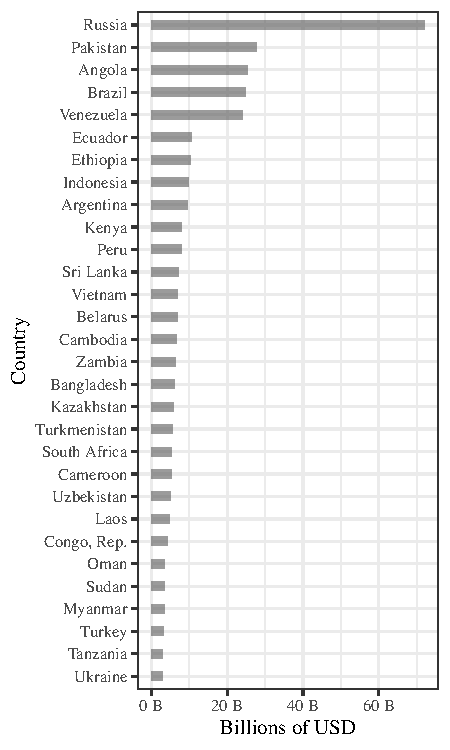
\includegraphics[width = \textwidth]{fig/total_debt.pdf}
        \caption{Top 30 Debtor by Total Debt in USD}
        \label{fig:total-debt-30}
    \end{subfigure}%
    ~
    \begin{subfigure}[t]{0.45\textwidth}
        \centering
        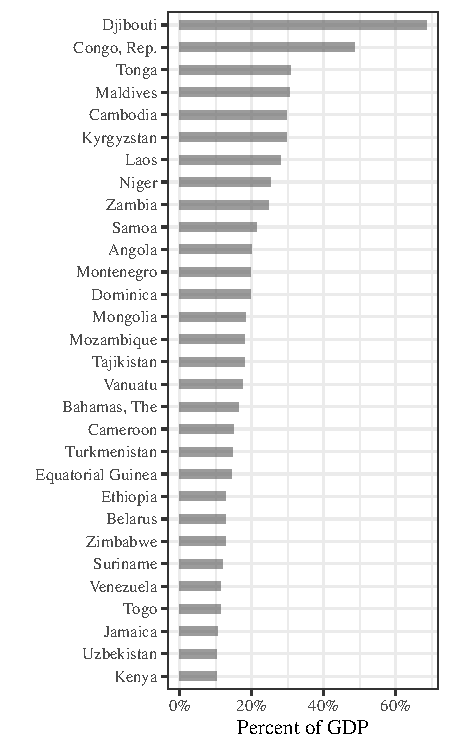
\includegraphics[width = \textwidth]{fig/perc_debt.pdf}
        \caption{Top 30 Debtor by Dept-to-GDP Ratio}
        \label{fig:perc-debt-30}
    \end{subfigure}
    \caption{Debt to China Statistic by Country in 2017}
    \label{fig:Country-Agg}
    \floatfoot{Source: HRT Database \citeyearpar{Horn-Reinhart-Trebesch-21} \\
    Note: The figure on the left presents the top 30 countries in amount of total external debt to China in 2017. The figure on the right compares by the China-debt-to-GDP ratio.}
\end{figure}

The top 30 countries with the largest debts to China's official creditors are displayed in \autoref{fig:total-debt-30}. Notably, Russia owes China over \$70 billion, while Pakistan's debt amounts to \$27 billion, both topping the list. Brazil and Venezuela are among the top 10 countries with the highest debt to China in Latin America. Contrary to what many people believe, African countries have not borrowed much from China. However, if we consider the ratio of Chinese debt to GDP in \autoref{fig:perc-debt-30}, some African countries appear to be highly indebted to China. Djibouti, for instance, has an alarming ratio of 68.5\% of its GDP consisting of Chinese debt, while Tonga, Niger, and Zambia have ratios exceeding 10\%.
\begin{figure}
    \centering
    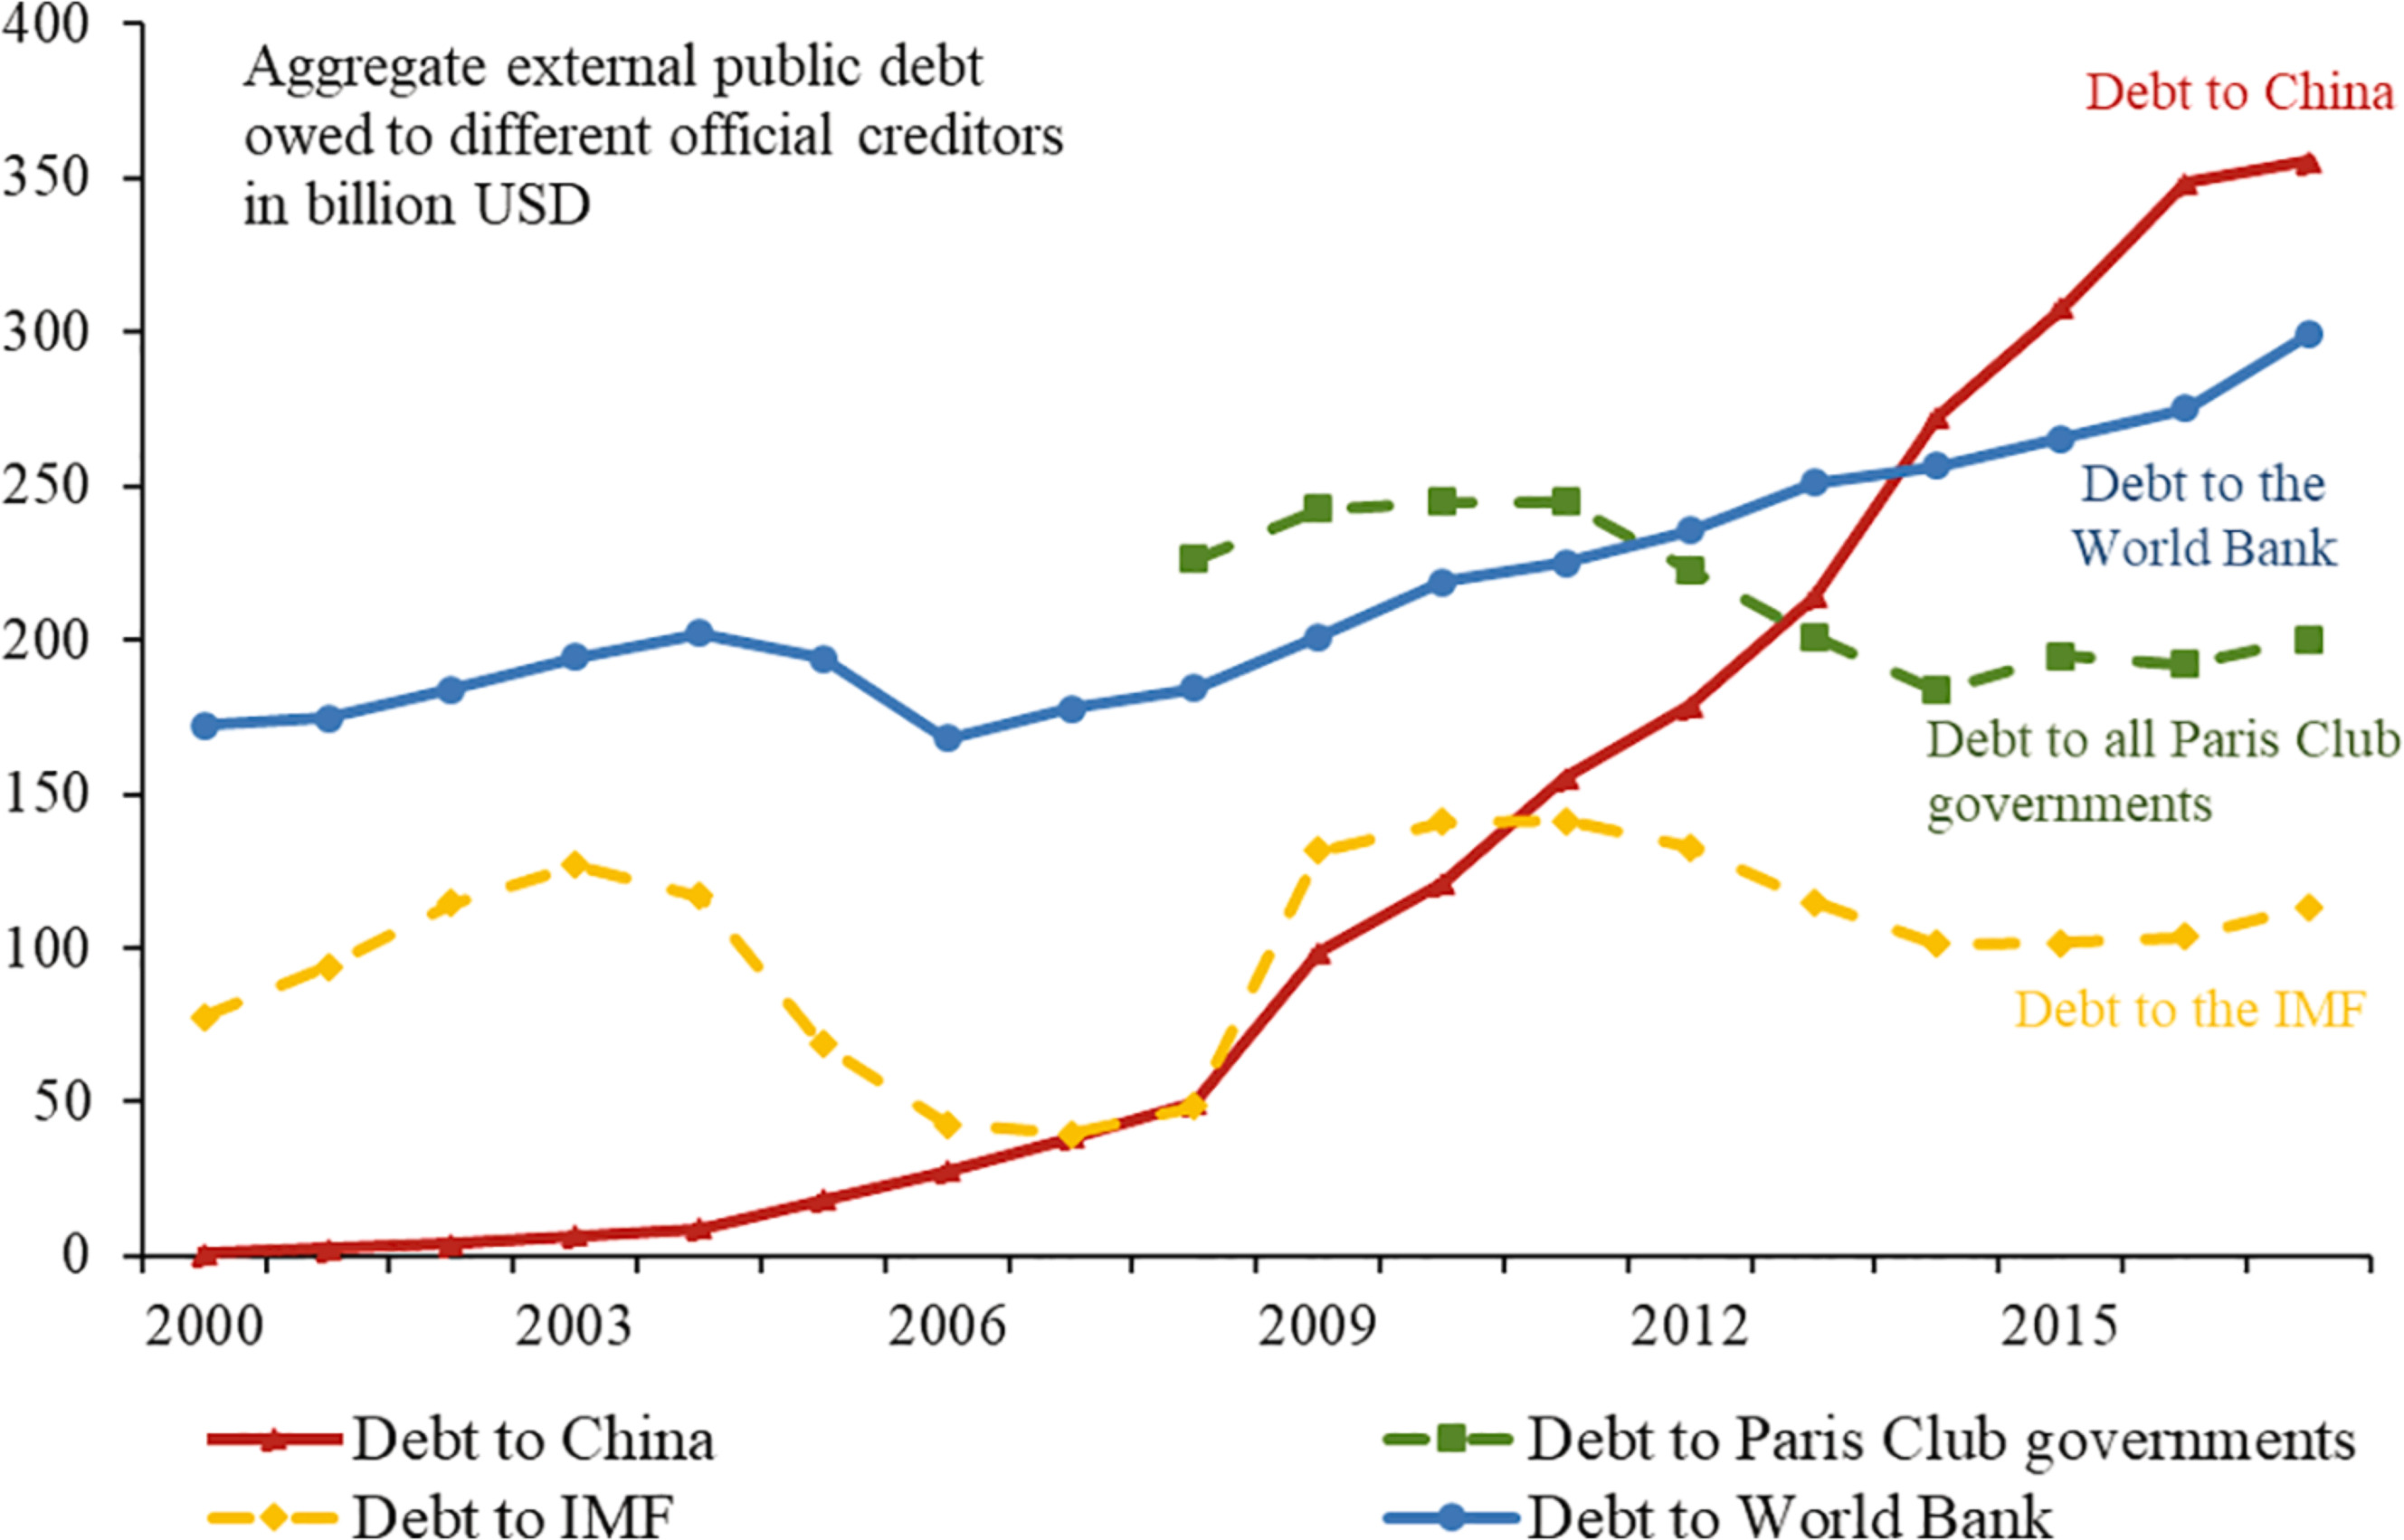
\includegraphics[width = 0.7\textwidth]{fig/temp-external-all-creditor.jpg}
    \caption{Change of Aggregate Public Debt for Different Official Creditors}
    \label{fig:debt-ts}
    \floatfoot{Source: HRT Database \citeyearpar{Horn-Reinhart-Trebesch-21} \\
    Note: The figure shows the change in the aggregate external public debt that the developing countries owed to different official creditors. These include China, World Bank (excluding China), IMF, and all 22 Paris Club governments. It is obvious that China had become the largest official creditors in the world according to the estimation of \citet*{Horn-Reinhart-Trebesch-21}.}
\end{figure}

A main finding in \citet*{Horn-Reinhart-Trebesch-21} is that China had become the world's largest creditor to developing countries after 2013, surpassing the amount of World Bank. \autoref{fig:debt-ts} shows the change of the total amount of debt from different main creditors, including China, World Bank\footnote{Including the International Development Association (IDA) and the International Bank for Reconstruction and Development (IBRD) }, IMF, and the aggregation of all countries in the Paris Club. The debt amount started to rise rapidly after 2000, when the China government launched the ``Go Out Policy'' in 1999. In 2017, the debt to China had reached \$355 billion, while the debt to World Bank was \$300 billion.


This database allows researchers to obtain the true amount of total debt of a country, and gauge the amount of debt that is considered superfluous and onerous for it.
For the next section, I briefly explain the two countries I will examine in my thesis, and demonstrate the importance of choosing it as a benchmark example.

\section*{Sri Lanka}
In the original article where the terminology ``Debt-trap Diplomacy'' was coined, \citet{Chellaney_2017} specifically mentioned the predicament faced by the Sri Lankan government. He argues that the Chinese government supported large infrastructure projects in Sri Lanka and provided heavy loans to their government, and as the project eventually failed to repay the debt, the country is then ensnared in the concessions to China. \autoref{fig: sri-lanka-debt-ts} shows the change in composition of the creditors to Sri Lanka.

The issue of the Hambantota port is regarded as a typical example of a debt-trap for some scholars~\citep*{Moramudali_2020}.
The construction of the port was initiated in 2007 and entrusted to the state-owned Chinese companies --- China Harbour Engineering Company and Sinohydro Corporation. The project was valued at \$361 million, of which Exim Bank financed 85\% at a yearly interest rate of 6.3\%\footnote{From AidData Project ID \#33409, ``China Eximbank provides \$306.7 million buyer's credit loan for Phase I of Hambantota''}.


China's involvement in Sri Lanka's infrastructure development was facilitated by President Mahinda Rajapaksa, during which China became Sri Lanka's leading investor and lender. This gave China significant diplomatic leverage over Sri Lanka. 
However, when Rajapaksa was unexpectedly defeated in the early 2015 election by Maithripala Sirisena, who campaigned on the promise to extricate Sri Lanka from the Chinese debt trap, work on major Chinese projects was suspended.

However, Sri Lanka's government was already on the brink of default, and Sirisena eventually acquiesced to a series of Chinese demands\footnotemark{}, including the sale of an 70\% stake in the Hambantota port to China Merchants Port (CM Port) and a 99-year lease.
\footnotetext{This narrative origins from \citet*{Chellaney_2017}. \citet*{Brautigam-meme-2020}, however, provides a different narrative. She mentioned that ``\emph{The proceeds were used to increase Sri Lanka's
US dollar reserves in 2017-18 with a view to the repayment of maturing international sovereign bonds \dots Therefore, the sale of Hambantota was originally a fire sale designed to raise money to deal
with larger debt problems.}''}
Notably, as argued by \citet*{Moramudali_2019}, the lease did not write off the loans obtained to construct Hambanota port. The proceeds from the lease were used to boost the country's dollar reserves in 2017-18, especially in preparation for the large amount of external debt that needed to be serviced when international sovereign bonds matured in early 2019. This means that the lease is not a debt-equity-swap, as common narratives elaborated \citep*{Moramudali_2020}.
Sri Lanka eventually declared a suspension on payment on most foreign debt from Aril 12, 2022. Whether Sri Lanka was indeed already under the extreme ``brink of default'' during 2015 is a major gap in the literature of sovereign default that has not yet been investigated.

\section*{Pakistan}
Similar to Sri Lanka, we observe the abrupt increase on the debt to China, as it already has a relatively high debt to other official creditors. \autoref{fig: pakistan-debt-ts} shows the change in composition of creditors to Pakistan. 
Pakistan is the centerpiece of the China Pakistan Economic Corridor (CPEC), a 3000 km corridor that connects China with the Arabian sea.
CPEC serves as an important network as it reduces the passage for China's energy import from the Middle Eastern countries \citep*{CPEC-wiki}.

China has launched enormous amounts of infrastructure in Pakistan after 2015. These items include a deep water port, road and rail lines, and most importantly, energy sector projects. Up to 2018, the estimation of the total value of projects under the CPEC is \$62 billion, out of which around \$33 billion is allocated for energy projects~\citep*{Hurley19-8-debt-trap}. China is expected to finance about 80 percent of this amount. The private investments for energy projects in Pakistan will be financed by the Exim Bank of China at an interest rate of 5-6\%. 
Private Independent Power Producers (IPP) will be responsible for constructing the energy projects under CPEC, instead of the governments of China or Pakistan. In turn, the government of Pakistan will be legally bound to buy electricity from these companies at rates that were agreed upon before.
However, despite this significant investment, some projects have already been cancelled, such as three major road projects that were cancelled at the end of 2017 \citep*{Hurley19-8-debt-trap}.

In the case of Pakistan, the sudden increase of debt to China draws the attention of researchers and journalists. For example, a report from the Financial Time titled ``Pakistan is on the brink'' states that Pakistan is following Sri Lanka into default. Given the recent frequent analogy drawn between Pakistan and Sri Lanka, it is essential to analyze Pakistan from the perspective of the sovereign default model.

  \label{ch:intro}
\chapter{Literature Review} \label{ch:lit}
\chapter{Analytic Model} \label{ch:model}
International debt often lacks perfect enforcement, and governments hold the decision of whether to repay the debts or default, based on the comparison of future values \citep*{Eaton-Gersovitz-81}. Therefore, default can be considered an optimal policy for a country that faces unsustainable debt levels. By defaulting, the country avoids the burden of paying interest on the debt, but it also faces the consequence of being excluded from the international credit market for a period of time. As a result, the country would have to rely solely on its own financial resources until it regains access to international credit markets.
Moreover, studies have pointed out that sovereign debt defaults are often accompanied by a devaluation of the currency; \citet*{Reinhart02} refers to this phenomenon as ``Twin Ds.''
Empirical analysis by \citet*{Na-18} further observes that the devaluation rate often decreases after the time of default, suggesting that the Twin Ds phenomenon is the joint result of an optimal policy.
They proposed a model that incorporates two key frictions: limited commitment to repay external debts and downward nominal wage rigidity.
It is a decentralized version of the Eaton-Gersovitz sovereign debt model.
The model predicts that default will occur only after a series of increasingly negative output shocks. Prior to default, domestic absorption experiences a severe contraction, which leads to a decline in demand for labor. However, due to downward nominal wage rigidity, real wages fail to adjust downward, resulting in involuntary unemployment. To prevent this situation, the optimal policy is to devalue the domestic currency, thereby reducing the real value of wages. As a result, both the model and the data show that default episodes are usually accompanied by significant currency devaluations \citep*{Na-18}.

For the sovereign debt model, I closely follow \citet*{Na-18} to replicate the stylized facts about sovereign debt defaults and examine the set of conditions under which default is the optimal decision.
The calibrated model will then serve as a benchmark metric that allows us to investigate whether China has potentially trapped heavily indebted poor counties into default, using the approach proposed by \citet*{Hinrichsen_2020-chapter4}.

\section{Households}
The model assumes that the economy is populated by a large number of representative households who maximize their expected lifetime utility
\begin{equation}
    \label{eq:utility}
    E_0 \sum_{t=0}^\infty \beta^t U(c_t),
\end{equation}
where $\beta \in(0,1)$ denotes the discount factor,
and $c_t$ represents the consumption good, which is composed of
tradable consumption $c_t^T$ and nontradable consumption $c_t^N$.
Assume that $c_t$ follows an aggregate technology
\begin{equation}
    \label{eq:A}
    c_t = A(c^T_t, c^N_t),
\end{equation}
where $A$ is an increasing, concave, and linearly homogeneous function that captures characteristics such as the ratio or elasticity of substitution between tradable and nontradable consumption.
The period utility function $U(c_t)$ follows the standard assumption, which is a strictly increasing and strictly concave function.

Assume that households only have access to the one-period and state non-contingent bond.
The households spend on consumption of tradable and untradable goods, along with their debt which is realized at this period. Their resources consist of labor incomes, dividend incomes, lump-sum transfers, as well as debt incomes. The households are also endowed with tradable goods, which follow a stochastic process.
The budget constraint of the representative household is then
\begin{equation}
    \label{eq:bc}
    P^T_t c^T_t + P^N_t c^N_t + P^T_t d_t =
    P^T_t \tilde{y}^T_t + W_t h_t + (1- \tau^d_t)P^T_t q^d_t d_{t+1} + F_t + \Phi_t,
\end{equation}
where $P^T_t (P^N_t)$ denotes the nominal price of tradable (nontradable) goods, $d_t$ the bond denominated in tradable goods which is due in period $t$, $q_t$ the price of debt to be repaid at $t+1$, $\tilde{y}^T_t$ the endowment of traded goods to the household, $W_t$ the nominal wage, $h_t$ the hours worked, $\tau^d_t$ the tax on debt, $F_t$ a lump-sum transfer from the government, and finally $\Phi_t$ the nominal profits from owning firms.
Households' working hour is bounded by an upper limit
\begin{equation}
    \label{eq:h-constraint}
    h_t \le \bar{h},
\end{equation}
and they take the working hours $h_t$ as given.

The households' problem is to choose $\{c_t, c_t^T, c_t^N, d_{t+1}\}$ such that their utility \eqref{eq:utility} is maximized subjected to the budget constraints \eqref{eq:A} -- \eqref{eq:h-constraint} and the no-Ponzi-game debt limit.
Further denote the relative price of nontradable in terms of tradable goods as $p_t \equiv \frac{P^N_t}{P^T_t}$, we have the following first order conditions
\begin{subequations}
    \begin{align}
        p_t &= \frac{A_2(c_t^T, c_t^N)}{A_1(c_t^t, c_t^N)}\\
        \lambda_t &= U'(c_t)A_1(c_t^T, c_t^N)\\
        (1-\tau_t^d)q_t^d \lambda_t &= \beta E_t \lambda_{t+1},
    \end{align}
\end{subequations}
where $\lambda_t$ is the Lagrange multiplier.

\section{Firms}
Perfectly competitive firms produce nontradable goods $y^N_t$ according to the production technology
\begin{equation}
    \label{eq:production}
    y^N_t = F(h_t),
\end{equation}
where $F$ is strictly increasing and strictly concave. Each firm maximizes its profit by choosing the amount of labor. Profit is given by
\begin{equation}
    \label{eq:profit}
    \Phi_t(h_t) = P^N_t F(h_t) - W_t h_t,
\end{equation}
and the optimal labor demand is then
\begin{equation*}
    P^N_t F'(h_t) = W_t.
\end{equation*}
Dividing both side by the price of tradable goods, and define $w_t \equiv \frac{W_t}{P^T_t}$ as the real wage in terms of tradable goods, the first order condition can be written as
\begin{equation}
    \label{eq:firm-FOC}
    p_t F'(h_t) = w_t.
\end{equation}

\section{Downward Nominal Wage Rigidity}
The key assumption in \citet*{Schmitt-Uribe-16} and \citet*{Na-18} is the downward nominal wage rigidity.
As the wage is unable to be adjusted to a lower level, involuntary unemployment is inevitable, hence the government has the incentive to allow devaluation. The model imposes a lower bound to the growth rate of nominal wage
\begin{equation}
    W_t \ge \gamma W_{t-1}, \qquad \gamma > 0.
\end{equation}
This implies that the growth rate $\frac{W_{t} - W_{t-1}}{W_{t-1}} \ge \gamma - 1$. When this inequality is unbinding ($W_t > \gamma W_{t-1}$), the economy is fully employed ($h_t = \bar{h}$). However, if the condition binds, the economy might have unemployment ($h_t < \bar{h}$). This relationship can be written as the following equation
\begin{equation}
    \label{eq:wage-rigid}
    (\bar{h} - h_t)(W_t - \gamma W_{t-1}) = 0.
\end{equation}


\section{Government}
I assume here, under the lack of enforcement in the international credit market that the government has the option to benevolently free up its domestic balance sheet by choosing to default or not.
Denote $I_t$ as the indicator of whether the government chooses to honor its debt in period $t$. If the government repays in this period ($I_{t} = 1$), then the country will be able to borrow in the following period, and hence $d_{t+1} > 0$. However, if the government chooses to default ($I_t = 0$), then the country will enter the status of financial autarky and is unable to have any sovereign debt in the next period, hence $d_{t+1} = 0$. The above scenario can be written as a slackness condition:
\begin{equation}
    \label{eq:gov-next-debt}
    (1 - I_t)d_{t+1} = 0 .
\end{equation}

To model the duration of financial exclusion, assume that once the country is in bad standing in the international credit market, it can regain a fiscally sound reputation and access to financial markets with probability $\theta \in [0,1)$, and remain in bad standing with probability $1-\theta$. This implies that the country has an average exclusion duration of $\frac{1}{\theta}$ periods.\footnote{
    The expected exclusion period $= \sum_{t=1}^{\infty} t \theta (1-\theta)^{t-1} = \theta  \sum_{t=1}^{\infty} t (1-\theta)^{t-1} = \frac{1}{\theta}$.
}

Assume that the government distributes the proceeds from the debt tax to households as a lump-sum payment. If the government honors the debt, then it repays $d_t$, but if the government decides to default, then it will not make any payments to foreign lenders, and instead will return any payments made by households directly to them. The budget constraint for the government can then be expressed as:
\begin{equation}
    \label{eq:gov-budget}
    f_t = \tau_t^d q_t^d d_{t+1} + (1-I_t)d_t,
\end{equation}
where $f_t \equiv \frac{F_t}{P^T_t}$ is the lump-sum transfer in terms of tradable goods. The right-hand side of the equation states that the transfer to households will include $d_t$ when $I_t = 0$, which is when the country decides to default. Nevertheless, the transfer of debt tax will be zero after default since $d_{t+1} = 0$ when $I_t = 1$, according to Equation \eqref{eq:gov-next-debt}.

\section{Foreign Lenders}
The behavior of foreign lenders is not explicitly modeled in this framework, but as all rational agents, the expected marginal utility of lending to the domestic country must be equivalent to the opportunity cost of funds.
Let $r^*$ represent the opportunity cost for the foreign lenders; this could be the world interest rate. Since $q_t$ is the price of debt that repays one unit of $d_{t+1}$ tomorrow, the return on the debt is $\frac{1}{q_t}$. The lenders take the risk of default into consideration, and hence the expected return will actually be lower. Assume that foreign lenders are risk neutral, this gives
\begin{equation}
    \label{eq:lender}
    \frac{\Pr(I_{t+1}=1 \mid I_{t}=1)}{q_t} = 1 + r^* .
\end{equation}

\section{Competitive Equilibrium}
Under equilibrium, households' consumption equals the production of firms:
\begin{equation}
    \label{eq:nontrade-clear}
    c^N_{t} = y^N_t.
\end{equation}
The tradable goods are purely endowed exogenously under an AR(1) process:
\begin{equation}
    \label{eq:ar1-output}
    \ln(y_t^T) = \rho \ln(y^T_{t-1}) + \mu_t,
\end{equation}
where $\mu_t \overset{\mathrm{iid}}{\sim} \mathcal{N}(0,\sigma_\mu^2)$ is an i.i.d. shock, and $ |\rho| \in [0,1)$ is the autocorrelation parameter.
When the country decides to default, it is in bad standing, and hence it faces an output loss defined by $L(y^T_t)$. The loss function is non-negative and increasing in the tradable goods. The endowment of tradable goods to the household is then:
\begin{equation}
    \label{eq:ytt}
    \tilde{y}^T_t =
        \begin{cases}
        y^T_t  - L(y^T_t) & \text{if } I_t = 0 \\
        y^T_t & \text{otherwise.}
        \end{cases}
\end{equation}
When the country defaults ($I_t = 0$), the endowment decreases.

The price of debt offered by foreign lenders $q_t$ should equal the price of the domestic debt $q^d_t$, but only during good standing:
\begin{equation}
    \label{eq:qq}
    I_t(q^d_t - q_t) = 0.
\end{equation}

The market-clearing condition can be established by combining various equations, including household budget constraints \eqref{eq:bc} and \eqref{eq:h-constraint}, the firm's production function \eqref{eq:production} and profit equation \eqref{eq:profit}, the government's constraint on debt \eqref{eq:gov-next-debt} and lump-sum return \eqref{eq:gov-budget}, and the conditions from \eqref{eq:nontrade-clear}, \eqref{eq:ytt}, and \eqref{eq:qq}.
Eventually, the clearing condition for tradable goods is:
\begin{equation}
    \label{eq:market-clearing}
    c^T_t = y^T_t - (1 - I_t)L(y^T_t) + I_t(q_t d_{t+1} - d_t)
\end{equation}

Assume that the law of one price applies to tradable goods. The foreign currency price of tradable goods is denoted as $P^{T*}_t$, while the nominal exchange rate is represented by $\mathcal{E}_t$. The law of one price states that the price of tradable goods in the domestic currency is equal to the foreign currency price multiplied by the nominal exchange rate.
\begin{equation*}
    P^T_t = P^{T*}_t \mathcal{E}_t
\end{equation*}
This implies that the price of a tradable good should be the same in both domestic and foreign currency terms in an efficient market.

Without loss of generosity, the foreign-currency price of the tradable goods is normalized to 1 ($P^{T*}_t = 1$)
Hence, the nominal price for tradable goods can be expressed as the nominal exchange rate:
\begin{equation}
    \label{eq:price-exrate}
    P^T_t = \mathcal{E}_t.
\end{equation}
For convenience, I also define the devaluation rate of domestic currency as:
\begin{equation}
    \label{eq:devaluation-rate}
    \epsilon_t \equiv \frac{\mathcal{E}_t}{\mathcal{E}_{t-1}} = \frac{P^T_t}{P^T_{t-1}}.
\end{equation}
The conditions are now sufficient to define a competitive equilibrium.
\begin{definition}[Competitive Equilibrium in \citet{Na-18}]
    A competitive equilibrium is a set of stochastic processes $\left\{ c^T_t, h_t, w_t, d_{t+1}, \lambda_t, q_t, q^d_t \right\}$ satisfying:
    \begin{align}
    c^T_t &= y^T_t - (1 - I_t)L(y^T_t) + I_t(q_t d_{t+1} - d_t), \\
    (1 - I_t)d_{t+1} &= 0, \\
    \lambda_t &= U'(A(c^T_t, F(h_t)))A_1(c_t^T, c_t^N),\\
    (1-\tau_t^d)q_t^d \lambda_t &= \beta E_t \lambda_{t+1}, \\
    I_t(q^d_t - q_t) &= 0, \\
    \frac{A_2(c_t^T, F(h_t))}{A_1(c_t^t, F(h_t))} &= \frac{w_t}{F'(h_t)} , \\
   w_t &\ge \gamma\frac{w_{t-1}}{\epsilon_t},\\
   h_t &\le \bar{h},\\
   \left( h_t - \bar{h} \right) \left( w_t - \gamma\frac{w_{t-1}}{\epsilon_t}\right) &= 0, \\
    I_t \left[ q_t - \frac{E_t I_{t+1}}{1+r^*} \right] &= 0,
\end{align}
    given processes $\left\{ y^T_t, \epsilon_t, \tau^d_t, I_t \right\}$ and initial conditions $w_{-1}$ and $d_0$.
\end{definition}
As proven by \citet{Na-18}, if the government is able to set the devaluation rate and the tax on debt freely, then the stochastic process of the variables $\left\{ c^T_t, h_t, d_{t+1}, q_t \right\}$ can be determined by the process of $\left\{ y^T_t, I_t\right\}$ and the initial debt level $d_0$.

As discussed previously, the decision of $I_t$ is an optimal policy for the government due to a lack of commitment to repay debt in the international credit market. Furthermore, the default decision of the government in the next period $t+1$ is also affected by the current decision. To see this argument, first notice that the default decision in $t+1$ is determined by the state variables $\left\{ y^T_{t+1}, d_{t+1} \right\}$. However, $d_{t+1}$ is determined in period $t$, which means that the government in period $t$ understands that it is able to affect the default decision in $t+1$ via the choice of $d_{t+1}$. As $y^T_{t+1}$ follows a first-order Markov process, the expected value of $y^T_{t+1}$ is a function of $y^T_t$, and hence the expected value for the default decision on period $t$ is actually a function of $y^T$ and $d_{t+1}$.

Recall that the price for debt $q_t$ relates to the probability of default in the next period. According to Equation \eqref{eq:lender}, it can be expressed in the contemporary variables:
\begin{equation}
    q_t = q(y^T_t, d_{t+1}).
\end{equation}
On the one hand, this provides economic intuition that the government internalizes the fact that its choice of debt in the next period can affect the price of the debt. On the other hand, this clarifies the dependencies of variables in the value function.


\section{Default Decision}
Following the standard Eaton-Gersovitz framework, this model considers the following three value functions:
value of continuing to repay the debt $v^c$, value of being in good standing $v^g$, and value of being in bad standing $v^b$.

Under the period of being in good financial standing, the value for the government to continue repaying the debt is the maximum value of the utility gained by the households this period, plus the discounted value of being in a good financial standing, subject to the households' budget constraints. Formally,
\begin{equation}
    \begin{aligned}
        v^c(y^T_t, d_t) = \max_{\left\{ c^T_t, h_t, d_{t+1} \right\}} \quad
        &\left\{
            U\left(
                A\left(c^T_t, F(h_t)\right)
             \right)
             + \beta E_t
             v^g \left(
                y^T_{t+1}, d+{t+1}
              \right)
         \right\}\\
          \text{s.t} \quad& c^T_t + d_t = y^T_t + q(y^T_t, d_{t+1}) d_{t+1} \\
                    & h_t \le \bar{h}.
    \end{aligned}
\end{equation}
Where the first constraint is obtained by setting $I_t = 1$ in \refeq{eq:market-clearing}, and the second is the constraint on working hour.

If the country is in bad standing, the consumption on tradable goods experiences a loss. The government has probability $\theta$ of regaining access to international financial markets, and probability $1 - \theta$ of continuing in bad standing. During the period in bad standing, the country obtains no international borrowing, hence, the state variable for debt is excluded. Formally,
\begin{equation}
    \begin{aligned}
        v^b(y^T_t) = \max_{\left\{ h_t \right\}} \quad
        &\left\{
            U\left(
                A\left( y^T_t - L(y^T_t), F(h_t)\right)
             \right)
             + \beta E_t \left[
                \theta v^g \left(
                    y^T_{t+1}, 0
                \right)
                + (1-\theta) v^b \left(
                    y^{T}_{t+1}
                 \right)
            \right]
         \right\}\\
          \text{s.t} \quad& h_t \le \bar{h}.
    \end{aligned}
\end{equation}
The tradable consumption $c^T_t = y^T_t - L(y^T_t)$ again follows \refeq{eq:market-clearing} by setting $I_t = 0$, and is substituted explicitly into the value function.

If the country is in good standing, the government has the freedom to choose which is best for the country: to continue or to default. The decision is made by comparing the value functions of the two scenarios, given the current output shock for tradable goods and the current level of debt
\begin{equation}
    v^g(y^T_t, d_t) = \max\left\{
        v^c(y^T_t, d_t) ,
        v^b(y^T_t)
     \right\}.
\end{equation}

Define the default set $D(d_t)$ as the set of tradable-output levels $y^T_t$ examined by the government in period $t$, in which the government's optimal respond is to default. Formally,
\begin{equation}
    D(d_t) = \left\{ 
        y^T_t : v^b(y^T_t) > v^c(y^T_t, d_t)
     \right\}.
\end{equation}
In other words, given a current debt level $d_t$, if the government observes that $y^T_t$ is inside $D(d_t)$, it chooses to default.

Under rational expectations, the foreign lenders recognize the default set, hence the price for debt is determined by Equation \eqref{eq:lender}, given by
\begin{equation}
    q(y^T_t, d_{t+1}) =
    \frac{1 - \Pr\left\{ y^T_{t+1} \in D(d_{t+1}) \mid y^T_t \right\}}{1 + r^*}.
\end{equation}
Note that the price of debt enters the value function of continuing, $v^c(y^T_t, d_{t})$.

It is obvious that the optimal labor supply is $h_t = \bar{h}$ since all functions, $F, A, U$, are monotonic, which implies that under the freedom to choose the devaluation rate and the tax on debt, the government can ensure full employment. Denote $w^f(c^T_t)$ the equilibrium wage function under full employment given the consumption of tradable goods. Combining Equation \eqref{eq:firm-FOC} and the Euler equation in \eqref{eq:FOC-HH-1} and impose the optimal policy $h_t = \bar{h}$, we have
\begin{equation}
    w_t = w^f(c^T_t) \equiv \frac{A_2(c^T_t, F(\bar{h}))}{A_1(c^T_t, F(\bar{h}))} F'(\bar{h}).
\end{equation}
Knowing that the wage has downward nominal rigidity, the government sets the devaluation rate accordingly. The downward rigidity \eqref{eq:wage-rigid} states that
\begin{equation*}
    \gamma \le \frac{W_t}{W_{t-1}} = \frac{w_t}{w_{t-1}} \frac{P^T_t}{P^T_{t-1}} = \epsilon \frac{w_t}{w_{t-1}},
\end{equation*}
where the second equal sign comes from Equation \eqref{eq:devaluation-rate}. Substitute the wage under full employment, we get
\begin{equation}
    \epsilon_t \ge \gamma \frac{w_{t-1}}{w^f(c^T_t)}.
\end{equation}
This is the family of optimal devaluation policies. Following \citet{Na-18} and \citet*{Hinrichsen_2020-chapter4}, we assume that the government chooses the minimal devaluation target that stabilizes nominal wages, that is, $
    \epsilon_t = \gamma \frac{w_{t-1}}{w^f(c^T_t)}.
$
\chapter{Empirical Results}  \label{ch:result}
\chapter{Conclusion and Discussion} \label{ch:conclusion}



\backmatter
\phantomsection
\addcontentsline{toc}{chapter}{\bibname}
\bibliographystyle{econ}

% Your bibliography goes here
\bibliography{bib/ref.bib}

% \chapter{Appendix}
% \begin{appendices}
%   \section*{The Bitcoin Law}
%   \label{Ap-BitcoinLaw}
%   \input{sections/Append-BitcoinLaw.tex}
% \end{appendices}
\end{document}
